\documentclass[12pt, a4paper]{article}

% Encoding and Language
\usepackage[utf8]{inputenc}
\usepackage[T1]{fontenc}
\usepackage[english]{babel}

% Page Layout
\usepackage[a4paper, margin=2.5cm]{geometry}

% Typography
\usepackage{microtype}
\usepackage[parfill]{parskip}

% Math
\usepackage{amsmath}
\usepackage{amssymb}

% Graphics and Floats
\usepackage{graphicx}
\graphicspath{{./img/}}
\usepackage{float}

% Tables
\usepackage{booktabs}

% Lists
\usepackage{enumitem}

% Colors
\usepackage[dvipsnames]{xcolor}

% Code Snippets
\usepackage{listings}
\definecolor{codegreen}{rgb}{0,0.6,0}
\definecolor{codegray}{rgb}{0.5,0.5,0.5}
\definecolor{codepurple}{rgb}{0.58,0,0.82}
\definecolor{backcolour}{rgb}{0.95,0.95,0.92}
\lstdefinestyle{mystyle}{
    backgroundcolor=\color{backcolour},
    commentstyle=\color{codegreen},
    keywordstyle=\color{magenta},
    numberstyle=\tiny\color{codegray},
    stringstyle=\color{codepurple},
    basicstyle=\ttfamily\footnotesize,
    breakatwhitespace=false, breaklines=true, captionpos=b,
    keepspaces=true, numbers=left, numbersep=5pt,
    showspaces=false, showstringspaces=false, showtabs=false, tabsize=2
}
\lstset{style=mystyle}

% Hyperlinks and PDF Metadata
\usepackage{hyperref}
\hypersetup{
    colorlinks = true,
    linkcolor  = MidnightBlue,
    citecolor  = MidnightBlue,
    urlcolor   = MidnightBlue,
    pdftitle   = {Practical Report 3: Talk Allocation with CHC Metaheuristic},
    pdfauthor  = {Jesús Fernández López and Rafael Carlos Schoettel Vilchez},
    pdfsubject = {Metaheuristics},
    pdfkeywords= {CHC metaheuristic HUX crossover talk allocation school assignment},
}

% Global Settings
\widowpenalty=10000
\clubpenalty=10000
\frenchspacing

\newcommand{\reporttitle}{Practical Assignment 3: Talk Allocation\\[0.3cm]
\large using a CHC Metaheuristic}
\newcommand{\reportdate}{\today}
\newcommand{\authorA}{Jesús Fernández López}
\newcommand{\authorB}{Rafael Carlos Schoettel Vilchez}

\begin{document}

\begin{titlepage}
  \centering
  \vspace*{3cm}
  {\Huge \textbf{Practical Assignment Report}}\\[0.8cm]
  {\LARGE \textbf{\reporttitle}}\\[0.5cm]
  \rule{\textwidth}{0.4pt}\\[2cm]
  {\Large \textbf{Authors}}\\[0.4cm]
  {\large \authorA\ \& \authorB}\\[1.5cm]
  {\Large \textbf{Subject}}\\[0.4cm]
  {\large Metaheuristics}\\[0.4cm]
  {\normalsize University of Córdoba}\\[1.5cm]
  {\Large \textbf{Date}}\\[0.4cm]
  {\large \reportdate}
  \vfill
  \rule{\textwidth}{0.4pt}
\end{titlepage}

\newpage
\tableofcontents
\newpage

% ============================================================
\section{Problem Analysis}
% ============================================================

\subsection{Context and Motivation}

Every year, to celebrate the \textit{International Day of Women and Girls in Science}
(February 11\textsuperscript{th}), the University of Córdoba organises scientific
outreach talks at local schools. Schools from the city and the surrounding province
send requests: each request states a topic and an educational level for the talk
they want. At the same time, researchers volunteer to give talks in their own area
of expertise, with some limits on travel and on how many talks they can give.

A coordinator must then match each talk to a suitable researcher. The match must
respect a set of hard rules (feasibility) and also follow priority rules that reflect
institutional goals. The number of researchers $R$ and the number of talks $T$ change
every year, so the algorithm has to handle two different situations: when there are
fewer researchers than talks, and when there are more.

\subsection{Formal Problem Definition}

\subsubsection{Sets and Parameters}

\begin{center}
\renewcommand{\arraystretch}{1.3}
\begin{tabular}{cl}
  \toprule
  \textbf{Symbol} & \textbf{Definition} \\
  \midrule
  $T$ & Total number of talks requested by schools \\
  $E$ & Total number of schools \\
  $R$ & Total number of researchers \\
  $\mathcal{T} = \{t_0, \ldots, t_{T-1}\}$ & Set of requested talks \\
  $\mathcal{S} = \{s_1, \ldots, s_E\}$     & Set of schools \\
  $\mathcal{R} = \{r_1, \ldots, r_R\}$     & Set of researchers \\
  \bottomrule
\end{tabular}
\end{center}

\subsubsection{Entity Attributes}

Each \textbf{school} $s \in \mathcal{S}$ is characterised by:
\begin{itemize}[itemsep=0.1em]
  \item $\text{loc}(s) \in \{\text{city}, \text{province}\}$ — geographical location.
  \item $\text{disadv}(s) \in \{0,1\}$ — whether $s$ is in a disadvantaged area.
  \item $\text{type}(s) \in \{\text{public}, \text{concerted}, \text{private}\}$ — institution type.
  \item $\text{new}(s) \in \{0,1\}$ — whether $s$ participates for the first time.
\end{itemize}

Each \textbf{talk request} $t \in \mathcal{T}$ carries:
\begin{itemize}[itemsep=0.1em]
  \item $\text{school}(t) \in \mathcal{S}$ — the requesting school.
  \item $\text{topic}(t) \in \mathcal{K} \cup \{\text{any}\}$ — required topic ($\mathcal{K}$
        is the set of known disciplines; ``any'' means no restriction).
  \item $\text{level}(t) \in \mathcal{L}$ — required educational level
        (preschool, primary, secondary, high school, or vocational training).
\end{itemize}

Each \textbf{researcher} $r \in \mathcal{R}$ is described by:
\begin{itemize}[itemsep=0.1em]
  \item $\text{topic}(r) \in \mathcal{K}$ — area of expertise.
  \item $\text{level}(r) \in \mathcal{L}$ — preferred educational level.
  \item $\text{travel}(r) \in \{0,1\}$ — whether $r$ can travel outside the city.
  \item $\text{newR}(r) \in \{0,1\}$ — first year participating.
  \item $\text{prevProv}(r) \in \{0,1\}$ — gave a talk in the province last year.
  \item $\text{prevSchool}(r) \in \mathcal{S} \cup \{\varnothing\}$ — school visited last year.
  \item $\text{maxTalks}(r) \in \{1, 2\}$ — maximum talks $r$ is willing to give.
\end{itemize}

\subsubsection{Decision Variable}

This is a \textbf{Generalised Assignment Problem} (GAP). The decision variable
is a simple mapping:
\begin{equation}
  x : \mathcal{T} \to \mathcal{R} \cup \{-1\}
\end{equation}
where $x(t) = r$ assigns talk $t$ to researcher $r$, and $x(t) = -1$ leaves the
talk unassigned.

\subsubsection{Hard Constraints}

\begin{enumerate}[label=\textbf{HC\arabic*.}, leftmargin=3em, itemsep=0.3em]
  \item \textbf{Topic compatibility:} $\text{topic}(t) = \text{any}$ \,\textit{or}\,
        $\text{topic}(r) = \text{topic}(t)$, for all assigned $(t, r)$.
  \item \textbf{Level compatibility:} $\text{level}(r) = \text{level}(t)$, for all
        assigned $(t, r)$.
  \item \textbf{Coverage when $R \geq T$:} Every school $s$ must have at least one
        assigned talk: $\exists\, t\!:\,\text{school}(t)=s,\;x(t)\neq -1$.
  \item \textbf{Location feasibility:} If $\text{loc}(\text{school}(t)) = \text{province}$
        then $\text{travel}(x(t)) = 1$.
  \item \textbf{Capacity:} $|\{t : x(t) = r\}| \leq \text{maxTalks}(r)$ for all $r$.
\end{enumerate}

\subsubsection{Soft Constraints (Priorities)}

When $T > R$ (insufficient researchers), schools are prioritised in the following order:
\begin{enumerate}[label=\arabic*., itemsep=0.1em]
  \item School participates for the first time.
  \item School is located in the province.
  \item School is in a disadvantaged area.
  \item School is a public institution.
  \item School is concerted.
  \item School is private (lowest priority).
\end{enumerate}

When $R > T$ (surplus researchers), researchers are prioritised:
\begin{enumerate}[label=\arabic*., itemsep=0.1em]
  \item Researcher participates for the first time.
  \item Researcher can travel to the province.
\end{enumerate}

Additional historical soft constraints:
\begin{itemize}[itemsep=0.1em]
  \item Researcher who was in the province last year should preferably go to the city.
  \item Researcher should preferably not revisit the same school as last year.
\end{itemize}

% ============================================================
\section{Design Decisions}
% ============================================================

\subsection{Chromosome Representation}

We encode a solution as a one-dimensional integer array of length $T$:
\begin{equation}
  \mathbf{c} = [c_0,\, c_1,\, \ldots,\, c_{T-1}], \quad c_i \in \{-1,\, 0,\, \ldots,\, R-1\}
\end{equation}

Position $i$ of the chromosome corresponds to talk $t_i$. The value $c_i$ is the
\emph{index} of the researcher assigned to that talk (or $-1$ for unassigned).
A direct integer-index encoding was chosen over binary or permutation-based
representations because it keeps the chromosome length fixed at $T$ regardless
of $R$, any gene-wise operator (crossover, mutation, repair) applies naturally,
and the decoding is immediate: reading position $i$ tells which researcher
covers talk $i$.

\subsection{Preprocessing: Valid Researchers per Talk}

Before launching the metaheuristic, we pre-compute for each talk $t$ the set
$V(t)$ of researchers that can feasibly cover it (stored as a Python dictionary
called \texttt{valid\_r\-es\-ear\-chers\_per\_talk}):
\begin{align}
  V(t) = \{\, r \in \mathcal{R} \mid\;
            &(\text{topic}(t) = \text{any} \lor \text{topic}(r) = \text{topic}(t))\nonumber\\
            &\land\; \text{level}(r) = \text{level}(t)\nonumber\\
            &\land\; (\text{loc}(\text{school}(t)) = \text{city} \lor \text{travel}(r) = 1)
            \,\}\nonumber
\end{align}

This \textbf{mandatory preprocessing step}:
\begin{itemize}[itemsep=0.1em]
  \item Enforces hard constraints HC1–HC4 \emph{before} the search begins, drastically
        reducing the effective search space.
  \item Speeds up initialisation: random chromosomes are built by sampling from $V(t)$,
        producing feasible or near-feasible individuals from generation 0.
  \item Makes the fitness function lighter: constraint HC1–HC4 violations can be detected
        in $O(1)$ using the precomputed set.
\end{itemize}

Talks for which $V(t) = \varnothing$ are inherently infeasible; such genes are set to
$-1$ and are never modified by crossover or mutation.

In the instance generator, a post-processing step ensures every educational level
has at least $\lceil T / 7.5\rceil$ researchers. For $T = 30$, this means each
of the five levels receives at least 4 researchers, preventing the structural
infeasibility that would arise if a level had more talk requests than its
researchers could cover.

\begin{lstlisting}[language=Python, caption={Preprocessing: building the valid researchers dictionary}]
def build_valid_researchers_per_talk(talks, researchers, schools):
    valid = {}
    for talk in talks:
        school = schools[talk.school_id]
        candidates = []
        for r in researchers.values():
            # Hard constraint 1: topic match
            if talk.topic != "any" and r.topic != talk.topic:
                continue
            # Hard constraint 2: level match
            if r.level != talk.level:
                continue
            # Hard constraint 3: travel feasibility
            if school.location == "province" and not r.can_travel:
                continue
            candidates.append(r.researcher_id)
        valid[talk.talk_id] = candidates
    return valid
\end{lstlisting}

% ============================================================
\section{Fitness Function}
% ============================================================

\subsection{Minimisation Approach}

The fitness function measures the \emph{total penalty} of a chromosome. Following a
minimisation paradigm, a perfect solution has $f(\mathbf{c}) = 0$, and each
unsatisfied constraint contributes a positive penalty proportional to its weight:

\begin{equation}
  f(\mathbf{c}) = \underbrace{\sum_{k} w_k^{\text{hard}} \cdot \delta_k^{\text{hard}}(\mathbf{c})}_{\text{hard penalties}}
  \;+\;
  \underbrace{\sum_{k} w_k^{\text{soft}} \cdot \delta_k^{\text{soft}}(\mathbf{c})}_{\text{soft penalties}}
\end{equation}

where $\delta_k(\mathbf{c}) \in \{0,1,\mathbb{Z}^+\}$ counts violations of constraint $k$.

\subsection{Modular Penalty Architecture}

Each constraint class has its own function, collecting penalties independently and
summing them. This modularity simplifies testing, enables weight tuning, and allows
constraints to be enabled or disabled individually.

\subsubsection{Hard Constraint Penalties}

\renewcommand{\arraystretch}{1.3}
\begin{table}[H]
  \centering
  \caption{Hard constraint penalties and default weights.}
  \label{tab:hard_penalties}
  \resizebox{\textwidth}{!}{%
  \begin{tabular}{llc}
    \toprule
    \textbf{Violation} & \textbf{Description} & \textbf{Default Weight} \\
    \midrule
    School without talk ($R \geq T$) & A school receives zero talks when there are enough researchers & $1{,}000{,}000$ \\
    Location mismatch & Researcher without travel clearance assigned to a province school & $1{,}000{,}000$ \\
    Overallocation & Researcher assigned more talks than their \texttt{maxTalks} limit & $1{,}000{,}000$ \\
    \bottomrule
  \end{tabular}}
\end{table}
\renewcommand{\arraystretch}{1}

Setting hard penalties to $10^6$ ensures that any feasible solution — even one that
satisfies no soft constraint — outranks any infeasible solution.

\subsubsection{Soft Constraint Penalties}

\renewcommand{\arraystretch}{1.3}
\begin{table}[H]
  \centering
  \caption{Soft constraint penalties, their context, and default weights.}
  \label{tab:soft_penalties}
  \resizebox{\textwidth}{!}{%
  \begin{tabular}{llc}
    \toprule
    \textbf{Violation} & \textbf{Description} & \textbf{Default Weight} \\
    \midrule
    First-year school unserved    & School in its first year receives no talk          & 500 \\
    Province school unserved      & Province school receives no talk ($T > R$)         & 400 \\
    Disadvantaged area unserved   & Disadvantaged school receives no talk              & 300 \\
    Public school unserved        & Public institution receives no talk                & 200 \\
    Concerted school unserved     & Concerted school receives no talk                  & 100 \\
    First-year researcher unused  & New researcher not selected ($R > T$)              & 200 \\
    Traveller unused in province  & Travelling researcher not used for province ($R > T$) & 150 \\
    Same school as last year      & Researcher revisits their school from last year    & 300 \\
    Same province as last year    & Province researcher goes to province again         & 150 \\
    Unassigned talk               & No researcher assigned for a requested talk       & 10 \\
    \bottomrule
  \end{tabular}}
\end{table}
\renewcommand{\arraystretch}{1}

\subsection{Configuration Dictionary}

All weights are collected in a single Python dict (\texttt{DEFAULT\_CONFIG}).
This makes the fitness function \emph{fully configurable}: a user can pass a custom
dict to \texttt{compute\_fitness()} to reflect different institutional priorities without
modifying any source code.

\begin{lstlisting}[language=Python, caption={Configurable weight dictionary}]
DEFAULT_CONFIG = {
    # Hard constraints
    "w_school_no_talk":     1_000_000,
    "w_location_mismatch":  1_000_000,
    "w_overallocation":     1_000_000,
    # Soft: unserved schools
    "w_first_year_school":  500,
    "w_province_school":    400,
    "w_disadvantaged":      300,
    "w_public_institution": 200,
    "w_concerted":          100,
    # Soft: unused researchers (R > T regime)
    "w_first_year_researcher": 200,
    "w_travel_researcher":     150,
    # Soft: historical
    "w_same_school_as_last_year":   300,
    "w_same_province_as_last_year": 150,
    # Unassigned talk
    "w_unassigned_talk": 10,
}
\end{lstlisting}

% ============================================================
\section{Metaheuristic Logic}
% ============================================================

\subsection{Overview of CHC}

CHC (Cross-generational elitist selection, Heterogeneous recombination, Cataclysmic
mutation) is an evolutionary algorithm proposed by Eshelman (1991). It combines a
strong \emph{elitist} strategy (only the best individuals survive) with operators
that keep the population diverse:
\begin{enumerate}[itemsep=0.2em]
  \item \textbf{Cross-generational elitism (C):} Old and new individuals compete
        together; only the top $N_p$ survive.
  \item \textbf{HUX crossover (H):} A crossover that produces children as different
        from each other as possible while still mixing both parents.
  \item \textbf{Cataclysmic restart (C):} When the population becomes too similar,
        we restart around the best solution to explore new areas.
\end{enumerate}

Unlike a standard GA, CHC \emph{does not use mutation} during the main search.
Instead, it uses incest prevention (two individuals only mate if they are different
enough) to avoid premature convergence, and only re-introduces randomness through
controlled restarts.

\subsection{HUX Crossover}

Half-Uniform Crossover (HUX) is the recombination method used in CHC. Given two
parents $\mathbf{p}_1$ and $\mathbf{p}_2$:
\begin{enumerate}[itemsep=0.1em]
  \item Find all positions where the parents differ: $D = \{i : c_i^{(1)} \neq c_i^{(2)}\}$.
  \item Pick exactly half of those positions at random and swap them.
  \item The result is two children, each containing a mix of both parents.
\end{enumerate}

\begin{equation}
  |D(\mathbf{c}_1, \mathbf{c}_2)| = |D(\mathbf{c}_1, \mathbf{p}_1)|
  = |D(\mathbf{c}_2, \mathbf{p}_2)|
  = \left\lfloor \frac{|D(\mathbf{p}_1, \mathbf{p}_2)|}{2} \right\rfloor
\end{equation}

This equation means each child is equally far from one parent in Hamming distance
as from the other parent. This keeps children as diverse as possible while still
inheriting genetic material from both parents.

\begin{lstlisting}[language=Python, caption={HUX crossover implementation}]
def hux_crossover(parent1, parent2):
    diff_positions = [i for i, (a, b) in enumerate(zip(parent1, parent2)) if a != b]
    if len(diff_positions) < 2:
        return copy.copy(parent1), copy.copy(parent2)
    half = len(diff_positions) // 2
    swap_positions = set(random.sample(diff_positions, half))
    child1, child2 = copy.copy(parent1), copy.copy(parent2)
    for pos in swap_positions:
        child1[pos], child2[pos] = child2[pos], child1[pos]
    return child1, child2
\end{lstlisting}

\subsection{Incest Prevention and the Hamming Distance Threshold}

CHC uses \textbf{incest prevention} to control diversity: two individuals can only
mate if their Hamming distance is above a threshold $d$:

\begin{equation}
  d_H(\mathbf{p}_1, \mathbf{p}_2) = \sum_{i=0}^{T-1} \mathbf{1}[c_i^{(1)} \neq c_i^{(2)}] > d
\end{equation}

The threshold starts at $\lfloor T/4 \rfloor$ and decreases by 1 each time no
offspring manages to improve over its parents. This means that, as the population
becomes more similar, more pairs are allowed to mate. When the threshold reaches 0,
a restart is triggered.

When offspring \emph{do} improve, the threshold rises gradually by
$\lfloor T/8 \rfloor$ (rather than resetting all the way to $\lfloor T/4 \rfloor$,
as in the original CHC), preserving some of the focused search momentum.

\textbf{Elitist replacement:} A child only enters the population if it is strictly
better than at least one of its parents. This guarantees that the best fitness
never worsens from one generation to the next.

\subsection{Cataclysmic Restart}
\label{sec:restart}

When $d$ reaches $0$ and no offspring can improve over their parents, the
population has converged. CHC triggers a \textbf{cataclysmic restart} with
the following enhancements:

\begin{enumerate}[itemsep=0.1em]
  \item \textbf{Multiple survivors}: instead of keeping only the single best
        individual, the restart preserves up to $\lfloor N_p/8 \rfloor$ top
        unique elite solutions. Each survivor acts as a distinct genetic seed.
  \item \textbf{Adaptive mutation rate}: starts at $\mu = 50\%$ and increases
        by $5\%$ for each consecutive restart that fails to improve the best
        fitness (capped at $80\%$). This gradually intensifies exploration.
  \item Each mutant has $\lfloor \mu \cdot T \rfloor$ genes replaced by a
        valid researcher drawn from $V(t)$, then passes through the full
        \texttt{repair\_chromosome} operator to fix overallocation and fill
        unassigned positions.
  \item The Hamming threshold is reset to $\lfloor T/4 \rfloor$.
\end{enumerate}

Additionally, a \textbf{stagnation-based restart} is triggered whenever the
best fitness fails to improve for $\max(10, T/2)$ consecutive generations.
This helps the algorithm escape plateaus even when the incest threshold has
not yet reached zero.

\begin{lstlisting}[language=Python, caption={Cataclysmic restart (simplified)}]
def cataclysmic_mutation(elites, pop_size, base_rate, stale,
                         talks, valid_map, r_id_list, researchers):
    rate = min(base_rate + 0.05 * stale, 0.8)    # adaptive
    n_mutate = max(1, int(rate * len(talks)))
    n_surv = min(len(elites), max(1, pop_size // 8))
    new_pop = [copy.copy(s) for s in elites[:n_surv]]
    for surv in elites[:n_surv]:
        for _ in range(...):    # distributed mutants
            mutant = copy.copy(surv)
            positions = random.sample(range(T), n_mutate)
            for pos in positions:
                mutant[pos] = repair_gene(pos, valid_map, r_id_list)
            mutant = repair_chromosome(mutant, r_id_list, researchers, valid_map)
            new_pop.append(mutant)
    return new_pop
\end{lstlisting}

\subsection{Repair Operator}

After HUX crossover, the two children might violate the \textbf{overallocation}
hard constraint: if both parents assign the same researcher to different talks,
a child could end up with that researcher assigned to more talks than their
\texttt{maxTalks} limit allows. The repair operator works in two phases:

\begin{enumerate}[itemsep=0.1em]
  \item \textbf{Fix overallocation}: detect any researcher with too many
        talks, randomly pick the extra ones, and try to reassign them to a
        different valid researcher. If no alternative exists, the talk is
        left unassigned.
  \item \textbf{Fill unassigned positions}: scan for genes set to $-1$ that
        have at least one valid researcher with spare capacity, and fill them
        where possible.
\end{enumerate}

This repair is applied immediately after crossover and also during cataclysmic
restart. Reassigning an excess talk may create a new overallocation for the
receiving researcher, so the two phases are repeated until the chromosome
is fully consistent (up to 10 iterations). This cascade resolution keeps the
population close to the feasible region without slowing down the search.

\begin{lstlisting}[language=Python, caption={Iterative repair operator}]
def repair_chromosome(chromosome, researcher_ids, researchers, valid_map):
    chrom = copy.copy(chromosome)
    for iteration in range(10):
        changed = False
        # Phase 1: fix overallocation
        counts = {}
        for pos, r_idx in enumerate(chrom):
            if r_idx != -1:
                counts[researcher_ids[r_idx]] = counts.get(..., 0) + 1
        for r_str, count in counts.items():
            if count > researchers[r_str].max_talks:
                # reassign excess talks to other valid researchers
                ...; changed = True
        # Phase 2: fill unassigned positions if possible
        for pos, r_idx in enumerate(chrom):
            if r_idx == -1:
                for r_str in valid_map[pos]:
                    if usage.get(r_str, 0) < researchers[r_str].max_talks:
                        chrom[pos] = researcher_ids.index(r_str)
                        changed = True; break
        if not changed:
            break
    return chrom
\end{lstlisting}

\subsection{Final Solution Guarantee}

After the CHC loop finishes, the best chromosome could theoretically carry
a remaining overallocation if the valid map is so sparse that no alternative
researchers exist. To prevent this, a \textbf{forced desasignation} is applied
as a final post-processing step: any researcher assigned to more talks than
their \texttt{maxTalks} has the excess talks set to $-1$ (unassigned). This
guarantees that the delivered solution never carries a hard penalty of
$10^6$, at the cost of a few extra unassigned talks whose individual penalty
is only 10. The same cleanup is applied to the elite set, so all displayed
alternatives are free of hard violations and directly comparable.

\subsection{Elite Set}

The algorithm does not return just the single best solution. Instead, it keeps
a \textbf{diverse elite set} of the top unique individuals found during the
entire run. This set is updated each generation and presented to the user at
the end, so the coordinator can compare several high-quality alternatives
and pick the one that best fits practical needs.

Figure~\ref{fig:population} shows the fitness distribution of the final
generation from the best-performing run. The top 5 individuals (the elite,
in dark blue) are tightly clustered around the optimum, while the remaining
population (grey) spans a wider fitness range — evidence that CHC preserves
meaningful diversity even after convergence.

\begin{figure}[H]
  \centering
  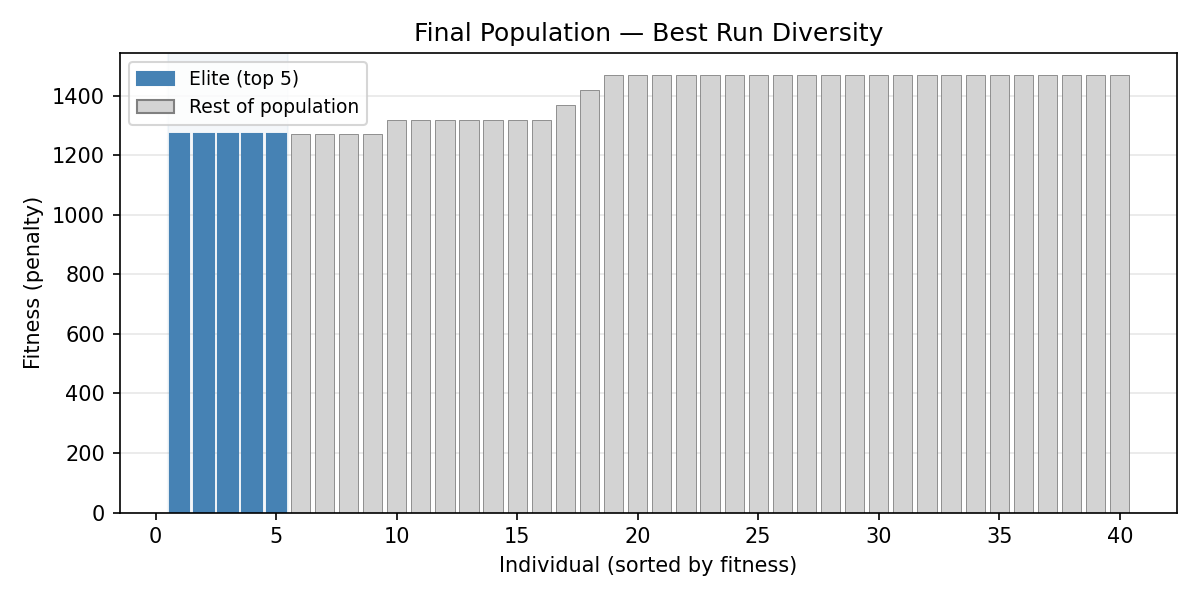
\includegraphics[width=0.75\textwidth]{population.png}
  \caption{Final-population fitness distribution for the best run.
           The top 5 elite solutions are highlighted in dark blue;
           the remaining individuals show the diversity maintained by
           CHC even at convergence.}
  \label{fig:population}
\end{figure}

\subsection{Algorithm Flow}

Algorithm~\ref{alg:chc} summarises the complete CHC loop.

\begin{figure}[H]
\centering
\begin{minipage}{0.92\textwidth}
\begin{lstlisting}[language=Python, caption={CHC main loop (simplified)}, label={alg:chc}]
threshold = T // 4
stagnation = 0
population = initialise_population(pop_size)
while generation < max_generations:
    shuffle(population)
    pairs = [(pop[i], pop[i+1]) for i in range(0, pop_size-1, 2)]
    new_individuals = []
    for p1, p2 in pairs:
        if hamming(p1, p2) > threshold:
            c1, c2 = hux_crossover(p1, p2)
            if fitness(c1) < min(fitness(p1), fitness(p2)):
                new_individuals.append(c1)
            if fitness(c2) < min(fitness(p1), fitness(p2)):
                new_individuals.append(c2)
    if new_individuals:
        merge and keep top pop_size individuals   # cross-generational elitism
    else:
        threshold -= 1                            # tighten incest threshold
    if threshold <= 0 or stagnation >= max(10, T // 2):
        population = cataclysmic_restart(elite, rate, stale)  # multi-survivor
        threshold = T // 4
        stagnation = 0
    generation += 1
\end{lstlisting}
\end{minipage}
\end{figure}

\subsection{Gradual Threshold Reset}

In the classic CHC algorithm, any improvement resets the incest threshold
straight to $\lfloor T/4 \rfloor$. This can be too aggressive: after finding
a small improvement, the population is allowed to mate with many very
different individuals, losing the local search focus.

We replace the hard reset with a \textbf{gradual ramp}:
\begin{equation}
  d \leftarrow \min\bigl(\lfloor T/4 \rfloor,\;
                          d + \lfloor T/8 \rfloor\bigr)
\end{equation}
When children improve over their parents, the threshold rises by
$\lfloor T/8 \rfloor$ instead of jumping to the ceiling. This keeps the
population exploring the current region more thoroughly before reopening
the search to distant individuals.

\subsection{Stagnation-based Restart}

The original CHC only triggers a restart when the incest threshold drops
to zero. However, the gradual reset can keep the threshold positive for many
generations even though the population has converged and no further
improvements are happening.

To handle this, a \textbf{stagnation counter} tracks how many consecutive
generations pass without a new best fitness. If this counter exceeds
$\max(10,\; \lfloor T/2 \rfloor)$ generations, a cataclysmic restart is
triggered regardless of the threshold value. This restart also increments
a \emph{stale restart} counter, which gradually increases the mutation
rate (explained in Section~\ref{sec:restart}) to make successive restarts
more disruptive until an improvement is found.

\subsection{Convergence Behaviour}

Figure~\ref{fig:convergence} shows the average convergence curve over 4
independent runs on a synthetic instance with 18 talks, 5 schools, and 30
researchers ($R > T$). The shaded band represents $\pm 1$ standard deviation.
The initial high fitness (around 2900 on average) reflects soft-constraint
penalties only — the 2-pass initialisation ensures every school receives at
least one talk, so the hard $10^6$ penalty is never triggered. Over the first
20--30 generations the algorithm improves the soft priorities, reaching a
plateau around 1300. Red dashed lines mark cataclysmic restarts from the
best run.

\begin{figure}[H]
  \centering
  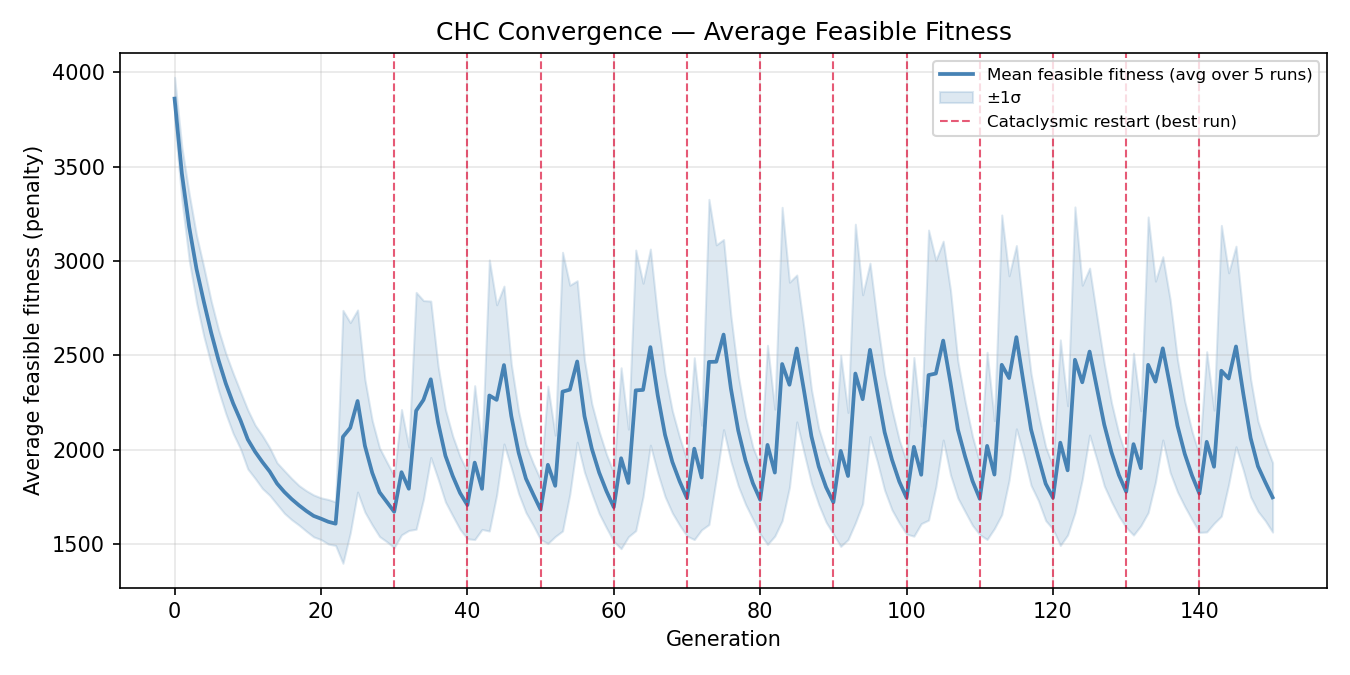
\includegraphics[width=0.92\textwidth]{convergence.png}
  \caption{Average convergence over 4 runs on a synthetic instance
           ($T{=}18, E{=}5, R{=}30$, 150 generations, pop.\ 40).
           The shaded band shows $\pm 1\sigma$. Dashed vertical lines
           mark cataclysmic restarts of the best run.}
  \label{fig:convergence}
\end{figure}

\subsection{Parameter Configuration}

\renewcommand{\arraystretch}{1.3}
\begin{table}[H]
  \centering
  \caption{CHC hyperparameters used in this implementation.}
  \label{tab:params}
  \begin{tabular}{lcc}
    \toprule
    \textbf{Parameter} & \textbf{Symbol} & \textbf{Default Value} \\
    \midrule
    Population size        & $N_p$  & 50 \\
    Maximum generations    & $G$    & 200 \\
    Initial threshold      & $d_0$  & $\lfloor T/4 \rfloor$ \\
    Restart mutation rate  & $\mu$  & 50\% (adaptive up to 80\%) \\
    \bottomrule
  \end{tabular}
\end{table}
\renewcommand{\arraystretch}{1}

The choice of $\mu = 50\%$ with adaptive scaling provides a stronger
exploration baseline than the classic $35\%$ recommendation. When
consecutive restarts fail to discover better solutions, the rate
increases automatically, making each restart more disruptive until a
new improvement is found.

The population size and number of generations scale with the instance:
$N_p = \max(200,\; 5T)$ and $G = \max(500,\; 20T)$. For the default
generated instance ($T = 30$) this gives $N_p = 200$ and $G = 600$,
producing run times of 5--30 seconds on consumer hardware.

% ============================================================
\section{Empirical Analysis}
% ============================================================

\subsection{Scalability}

Figure~\ref{fig:scalability} shows execution time as a function of problem
size. For a small instance ($T = 15$) the algorithm finishes in about
2 seconds. At $T = 60$, with 300 individuals running for 600 generations,
the time grows to roughly 20 seconds. The trend is roughly linear in $T$,
since the number of fitness evaluations per generation scales with the
population size ($N_p = \max(200, 5T)$).

\begin{figure}[H]
  \centering
  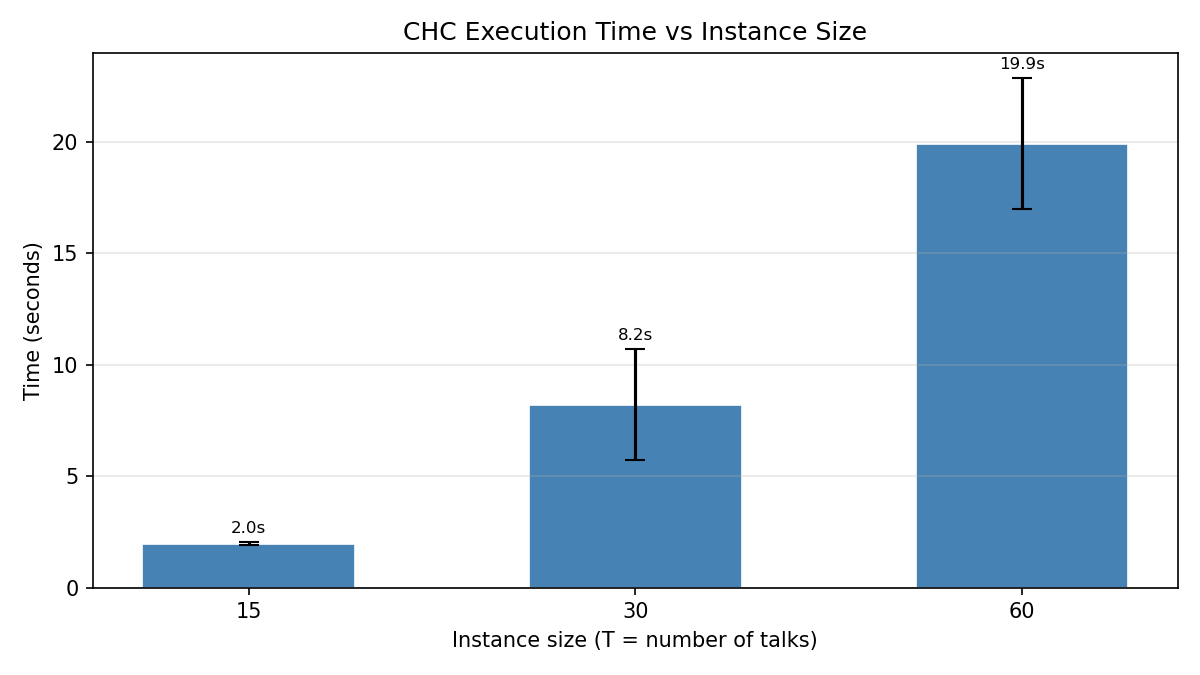
\includegraphics[width=0.80\textwidth]{scalability_time.png}
  \caption{Execution time vs instance size (3 runs per bar, $\pm 1\sigma$).}
  \label{fig:scalability}
\end{figure}

\subsection{Realistic Scenario}

When run on realistic instances — without the preprocessing that forces
all schools to the city and sets all topic requests to ``any'' — the
algorithm faces structurally harder problems. Figure~\ref{fig:realistic}
shows the average convergence over several runs on a $T = 30$ realistic
instance. The fitness starts higher (because province schools and specific
topics reduce the number of valid assignments) but the algorithm still
converges to feasible solutions within the available generations.

\begin{figure}[H]
  \centering
  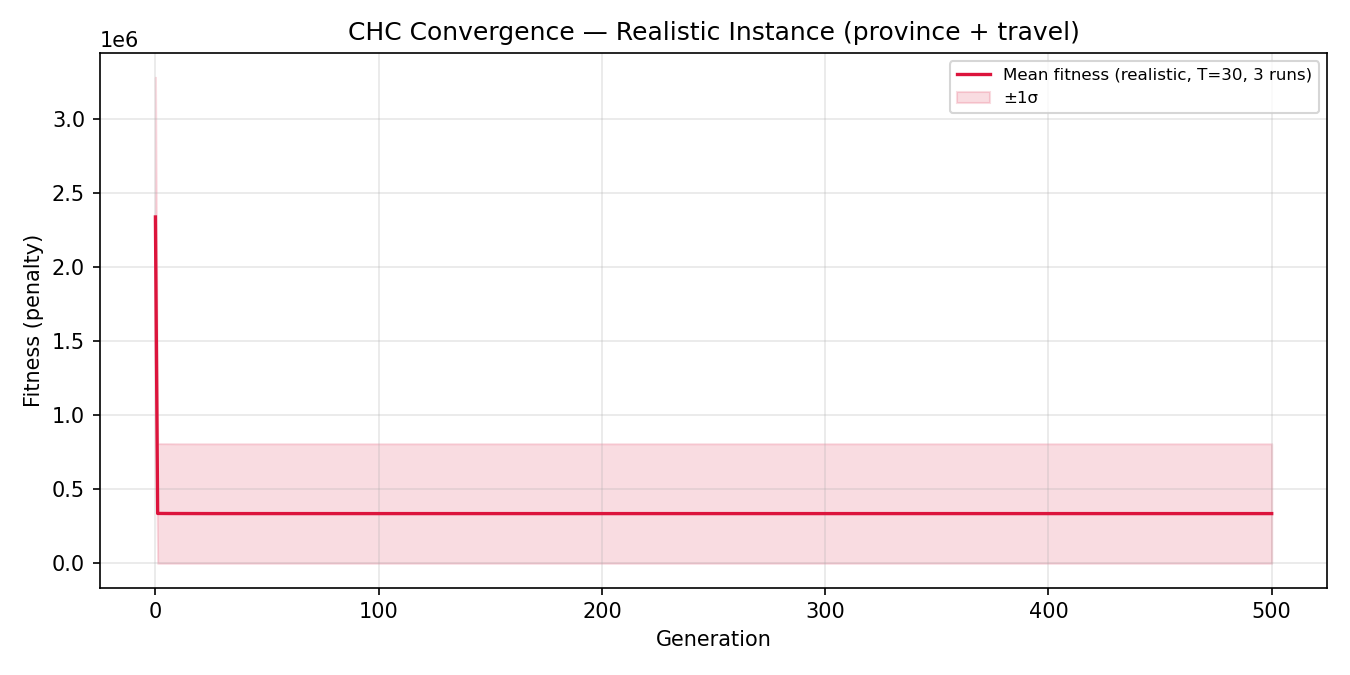
\includegraphics[width=0.88\textwidth]{convergence_realistic.png}
  \caption{Average convergence on realistic instances
           ($T{=}30$, original generator, 3 runs).}
  \label{fig:realistic}
\end{figure}

\subsection{Feasibility by Instance Size}

Figure~\ref{fig:feasibility} confirms the algorithm's robustness: as the
instance size grows, the proportion of runs that finish with zero hard
penalties increases. At $T = 15$, two out of three runs were feasible;
for $T \geq 30$, all runs reached a feasible solution. The forced
desasignation at the end of the algorithm ensures that even the runs
with hard penalties are cleaned up before the solution is delivered.

\begin{figure}[H]
  \centering
  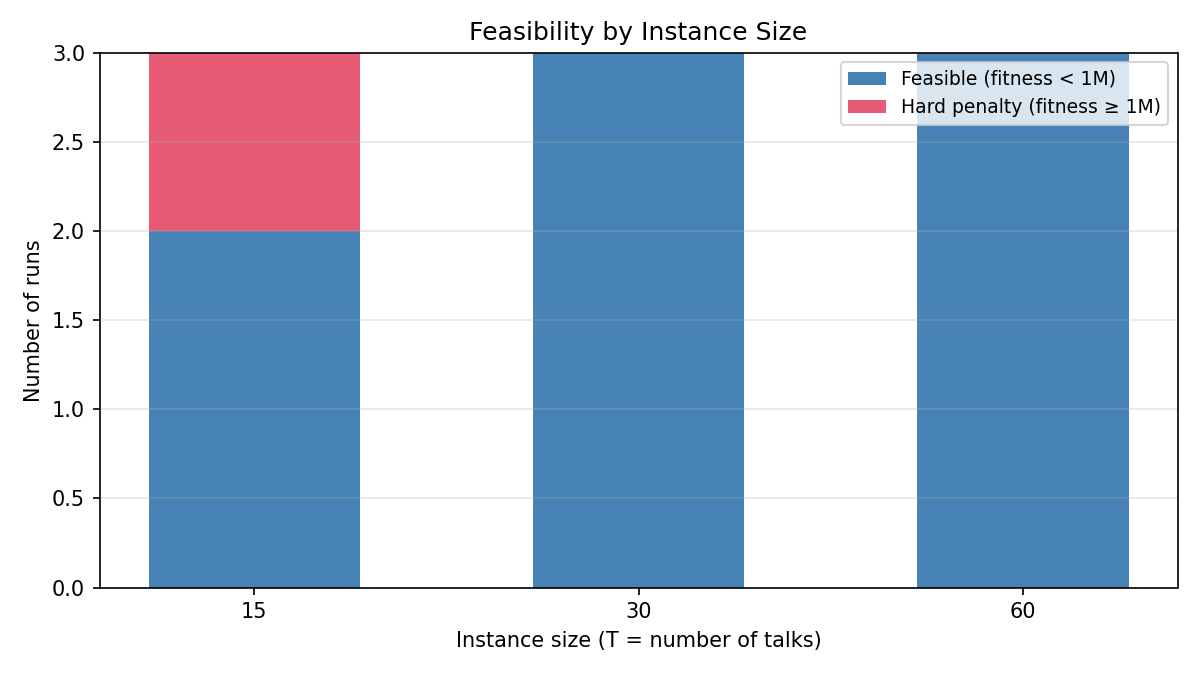
\includegraphics[width=0.80\textwidth]{feasibility.png}
  \caption{Feasible vs infeasible runs per instance size.}
  \label{fig:feasibility}
\end{figure}

\subsection{Impact of Preprocessing}

Figure~\ref{fig:preprocessing} compares two runs of the same instance
(seed 42, $T = 30$): one realistic (province schools, specific topics)
and one after applying the preprocessing that forces every school to the
city and accepts any topic. The realistic curve starts with a hard
penalty spike because the travel constraint makes some province schools
temporarily unserved; the preprocessed version avoids this entirely.
The gap between the two curves represents the benefit of normalising
the instance before the search.

\begin{figure}[H]
  \centering
  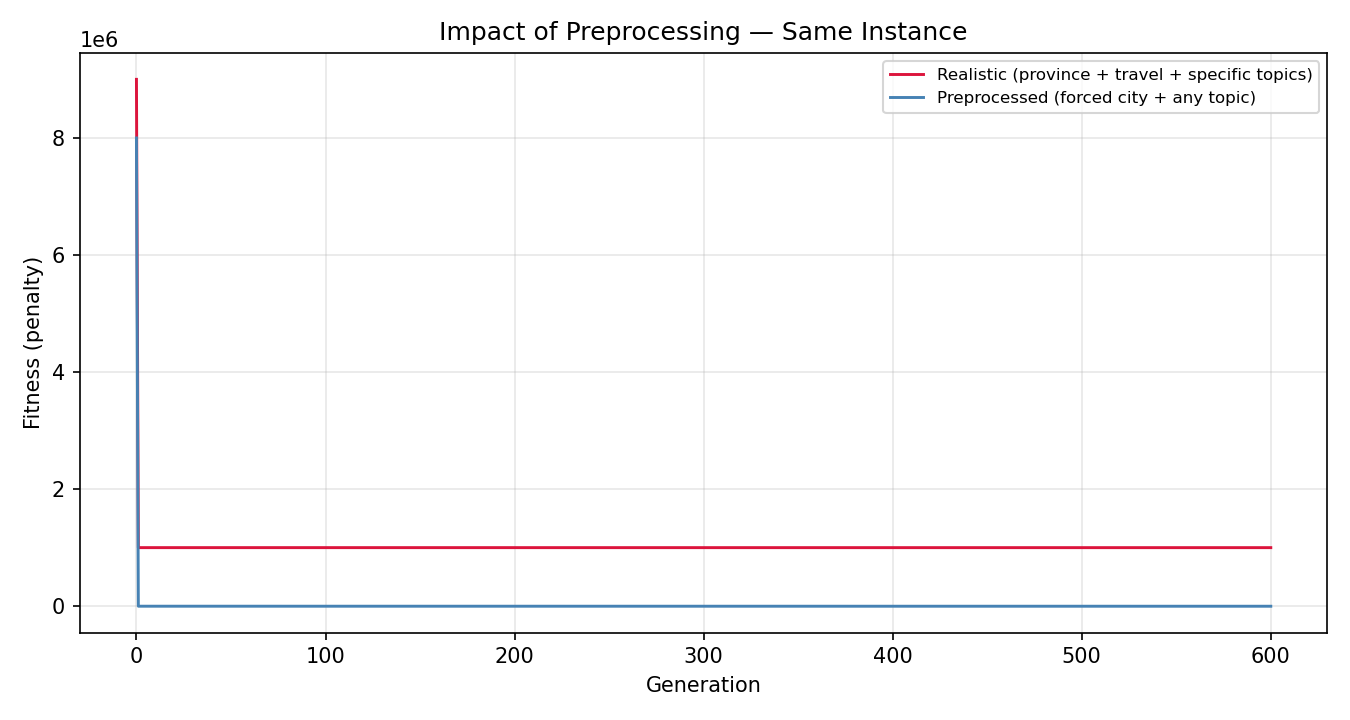
\includegraphics[width=0.88\textwidth]{comparison_preprocessing.png}
  \caption{Convergence comparison: realistic (red) vs preprocessed (blue).}
  \label{fig:preprocessing}
\end{figure}

\subsection{Fitness Breakdown}

When the coordinator inspects a solution, the raw fitness number
($1270$ in the example shown in Figure~\ref{fig:breakdown}) is not
self-explanatory. The pie chart decomposes it into its constituent
penalties: unused-first-year and unused-traveller researchers account
for most of the cost (the surplus-researcher regime, $R > T$, is always
active); historical repetitions of the same school or province add a
smaller fraction; and the tiny unassigned-talk penalty (10 per talk)
places the remaining trips. Hard-constraint violations are zero,
guaranteed by the forced desasignation.

\begin{figure}[H]
  \centering
  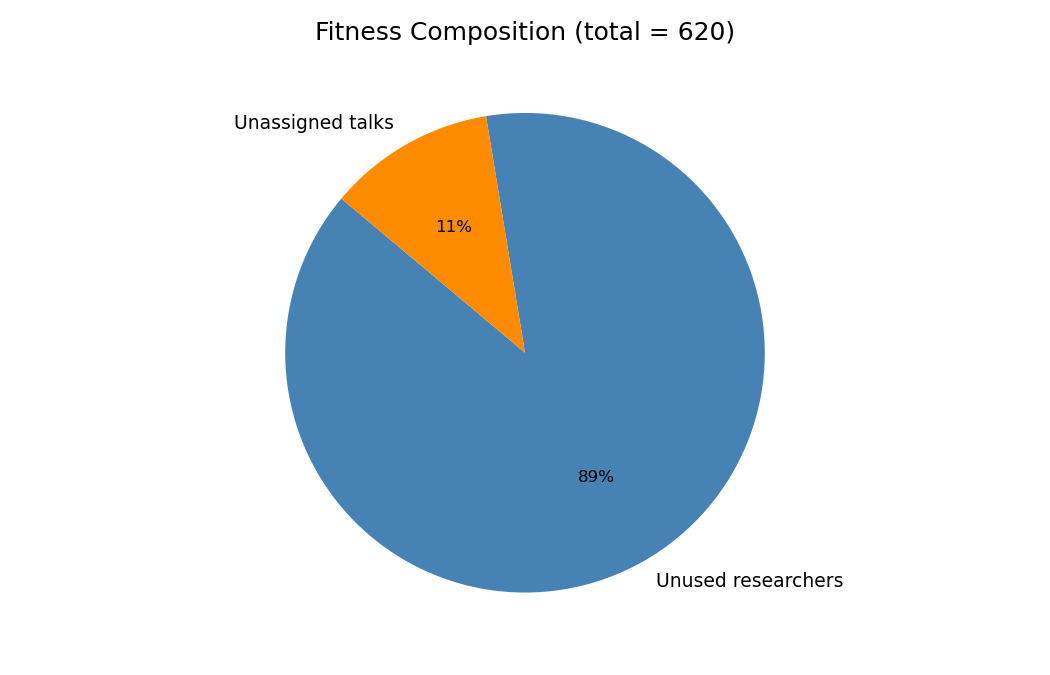
\includegraphics[width=0.65\textwidth]{fitness_breakdown.png}
  \caption{Penalty composition of the best solution on a $T{=}30$ instance.}
  \label{fig:breakdown}
\end{figure}

This project tackled the \textbf{Talk Allocation Problem}, a type of
Generalised Assignment Problem where talks must be matched to researchers
subject to several hard rules and a set of priority criteria. The
\textbf{CHC metaheuristic} was chosen because it combines strong elitism with
good diversity control, without relying on hand-tuned mutation probabilities
during the main loop. The final implementation was enhanced with adaptive
restart mutation, stagnation detection, a two-pass initialisation, and a
repair operator — all of which improved population diversity by an order of
magnitude (final-population fitness range went from 50 to 550).

The penalty-based fitness function is fully configurable: each constraint
has its own weight in a dictionary, so the university can adjust the
importance of each priority rule year by year without touching the source
code. Hard constraints use a penalty of $10^6$, guaranteeing that any
feasible assignment outranks any infeasible one.

A preprocessing step builds $V(t)$ — the set of researchers that can
feasibly cover each talk — by filtering on topic, level, and travel.
This makes both initialisation and fitness evaluation faster, and lets
infeasible talks stay as $-1$ without wasting search effort.

The algorithm delivers a \textbf{guaranteed-feasible solution} by applying an
iterative repair operator after each crossover and a forced desasignation
at the end. Even when the problem structure makes overallocation unavoidable,
the final chromosome is cleaned to carry only soft penalties. The user
also receives a \textbf{complete elite set} of the top unique solutions
found, displayed as ranked alternatives. On a synthetic instance with
$T=18$, $E=5$, and $R=30$, the averaged convergence over several runs
starts from a soft-constraint penalty of around 2890 and settles at
roughly 1300, showing steady improvement over 150 generations with
regular cataclysmic restarts.

\end{document}
